%%%%%%%%%%%%%%%%%%%%%%% file template.tex %%%%%%%%%%%%%%%%%%%%%%%%%
%
% This is a template file for Web of Conferences Journal
%
% Copy it to a new file with a new name and use it as the basis
% for your article
%
%%%%%%%%%%%%%%%%%%%%%%%%%% EDP Science %%%%%%%%%%%%%%%%%%%%%%%%%%%%
%
%%%\documentclass[option comma separated list]{webofc}
%%%Three important options:
%%% "epj" for EPJ Web of Conferences Journal
%%% "bio" for BIO Web of Conferences Journal
%%% "mat" for MATEC Web of Conferences Journal
%%% "itm" for ITM Web of Conferences Journal
%%% "e3s" for E3S Web of Conferences Journal
%%% "shs" for SHS Web of Conferences Journal
%%% "twocolumn" for typesetting an article in two columns format (default one column)
\documentclass[epj,twocolumn]{webofc}
\usepackage[varg]{txfonts}   % Web of Conferences font
%
% Put here some packages required or/and some personnal commands
%
% Important: please activate and fill the "wocname" command with the exact title of the series for conferences not included in any of the series listed on the top
\usepackage{siunitx}
\usepackage{cleveref}
\usepackage{subcaption}
\captionsetup{compatibility=false}

% Very important: please fill the "woctitle" command with the exact title of the conference
%
\woctitle{Powders \& Grains 2017}
%
%
\begin{document}
%
\title{Collapse of tall granular columns in fluid}
%
% subtitle is optionnal
%
%%%\subtitle{Do you have a subtitle?\\ If so, write it here}

\author{\firstname{Krishna} \lastname{Kumar}\inst{1}\fnsep\thanks{\email{kks32@cam.ac.uk}} \and
        \firstname{Kenichi} \lastname{Soga}\inst{2}\fnsep\thanks{\email{soga@berkeley.edu}} \and
        \firstname{Jean-Yves} \lastname{Delenne}\inst{3}\fnsep\thanks{\email{}}
}

\institute{Department of Engineering, University of Cambridge, UK 
\and
           University of California, Berkeley, USA
\and
           INRA, France
}

\abstract{%
  Avalanches, landslides, and debris flows are geophysical hazards, involve
  rapid mass movement of granular solids, water, and air as a multi-phase
  system. In order to describe the mechanism of immersed granular flows,
  it is important to consider both the dynamics of the solid phase and the
  role of the ambient fluid~\cite{Denlinger2001}. In the present study,
  the collapse of a granular column in fluid is
  studied using 2D LBM - DEM. The flow kinematics are compared with the dry
  and buoyant granular collapse to understand the influence of hydrodynamic
  forces and lubrication on the run-out. In the case of tall columns,
  the amount of material destabilised above the failure plane is larger than
  that of short columns. Hence in tall columns, the surface area of the
  mobilised mass that interacts with the surrounding fluid is significantly
  higher than the short columns. This increase in the area of soil - fluid
  interaction results in an increase in the formation of turbulent vortices
  that alter the deposit morphology during the collapse. It is observed that
  the vortices result in the formation of heaps that significantly affect
  the distribution of mass in the flow. In order to understand the behaviour
  of tall columns, the run-out behaviour
  of a dense granular column with an initial aspect ratio of 6 is studied.
  The collapse of a tall granular column on slopes of 0, 2.5, 5 and 7.5
  are studied.}
%
\maketitle
%
\section{Collapse of granular columns}
The collapse of a granular column on a horizontal surface is a simple case
of granular flow, however a proper model that describes the flow dynamics
is still lacking. Experimental investigations have shown that the flow
duration, the spreading velocity, the final extent of the deposit, and the
energy dissipation can be scaled in a quantitative way independent of
substrate properties, grain size, density, and shape of the granular
material and released mass~\cite{Staron2007a, Lajeunesse2005, Lube2005}. 

Granular collapse on a horizontal plane exhibit two distinct flow regimes:
(a) for columns with aspect ratio ‘a’ <1.7 a linear relation between the
spread and aspect ratio can be observed, and (b) for ‘a’ > 1.7 a power-law
relationship exists.~\citet{Soundararajan2015} observed that a simple
frictional dissipation model is able to capture the flow dynamics for
columns with small aspect ratios. However, for tall columns the flow
dyanmics of is controlled by the initial collisional regime, resulting in a
power-law relationship with the aspect ratios. Simple mathematical models
based on conservation of horizontal momentum capture the scaling laws of
the final deposit, but fail to describe the initial transition regime
~\citep{Kumar2013}. Granular flow is modelled as a frictional dissipation
process in continuum mechanics but the lack of influence of inter-particle
collision and friction on the energy dissipation and spreading dynamics is
surprising.

\section{Tall columns}

In the case of tall columns, the amount of material destabilised above the 
failure plane is larger than that of short columns. Hence in tall columns, 
the surface area of the mobilised mass that interacts with the 
surrounding fluid is significantly higher than the short columns. This 
increase in the area of soil - fluid interaction results in an increase
in the formation of turbulent vortices that alter the deposit morphology during 
the collapse. It is observed that the vortices result in formation of heaps 
that significantly affect the distribution of mass in the flow.
~\citet{Staron2007a} observed that the 
distribution of mass in a granular flow plays a crucial role in the flow 
kinematics. In order to understand the behaviour of tall columns, the run-out 
behaviour of a dense granular column with an initial aspect ratio of 6 is 
studied. The collapse of a tall granular column on slopes of 0\si{\degree}, 
2.5\si{\degree}, 5\si{\degree} and 7.5\si{\degree} are studied. A hydrodynamic 
radius of \textit{r} = 0.85 \textit{R} is adopted. 

Snapshots of the collapse of an aspect ratio 6 column in fluid on a horizontal 
surface are shown in~\cref{fig:LBM_DEM_a6}. The initial stage of collapse is 
characterised by the free-fall of grains above the failure surface. Unlike the 
dry condition, as the grains undergo free-fall due to gravity, they interact 
with the surrounding fluid experiencing drag forces. This results in a 
significant drop in the kinetic energy available for the flow. As the grains 
reach the static region, they interact with the neighbouring grains and the 
kinetic energy gained during the free fall is converted into horizontal 
acceleration. Uniquely during this stage ($t = 3\tau_c$) the interactions 
between the soil grains on the surface with the surrounding fluid result in the 
formation of eddies. The number of eddies formed during the flow is 
proportional to the surface area of the granular mass interacting with the 
fluid. Hydroplaning can be observed at the flow front ($t = 3\tau_c$). Two 
large vortices with almost the same size can be observed at the final stage of 
collapse. The soil grains on the surface experience suction due to formation of 
eddies and this results in formation of heaps of granular mass in front of each 
vortex. The formation of heaps, although in evidence, doesn't significantly 
affect the distribution of mass in the case of collapse on a horizontal plane. 

\begin{figure}[htpb]
\centering
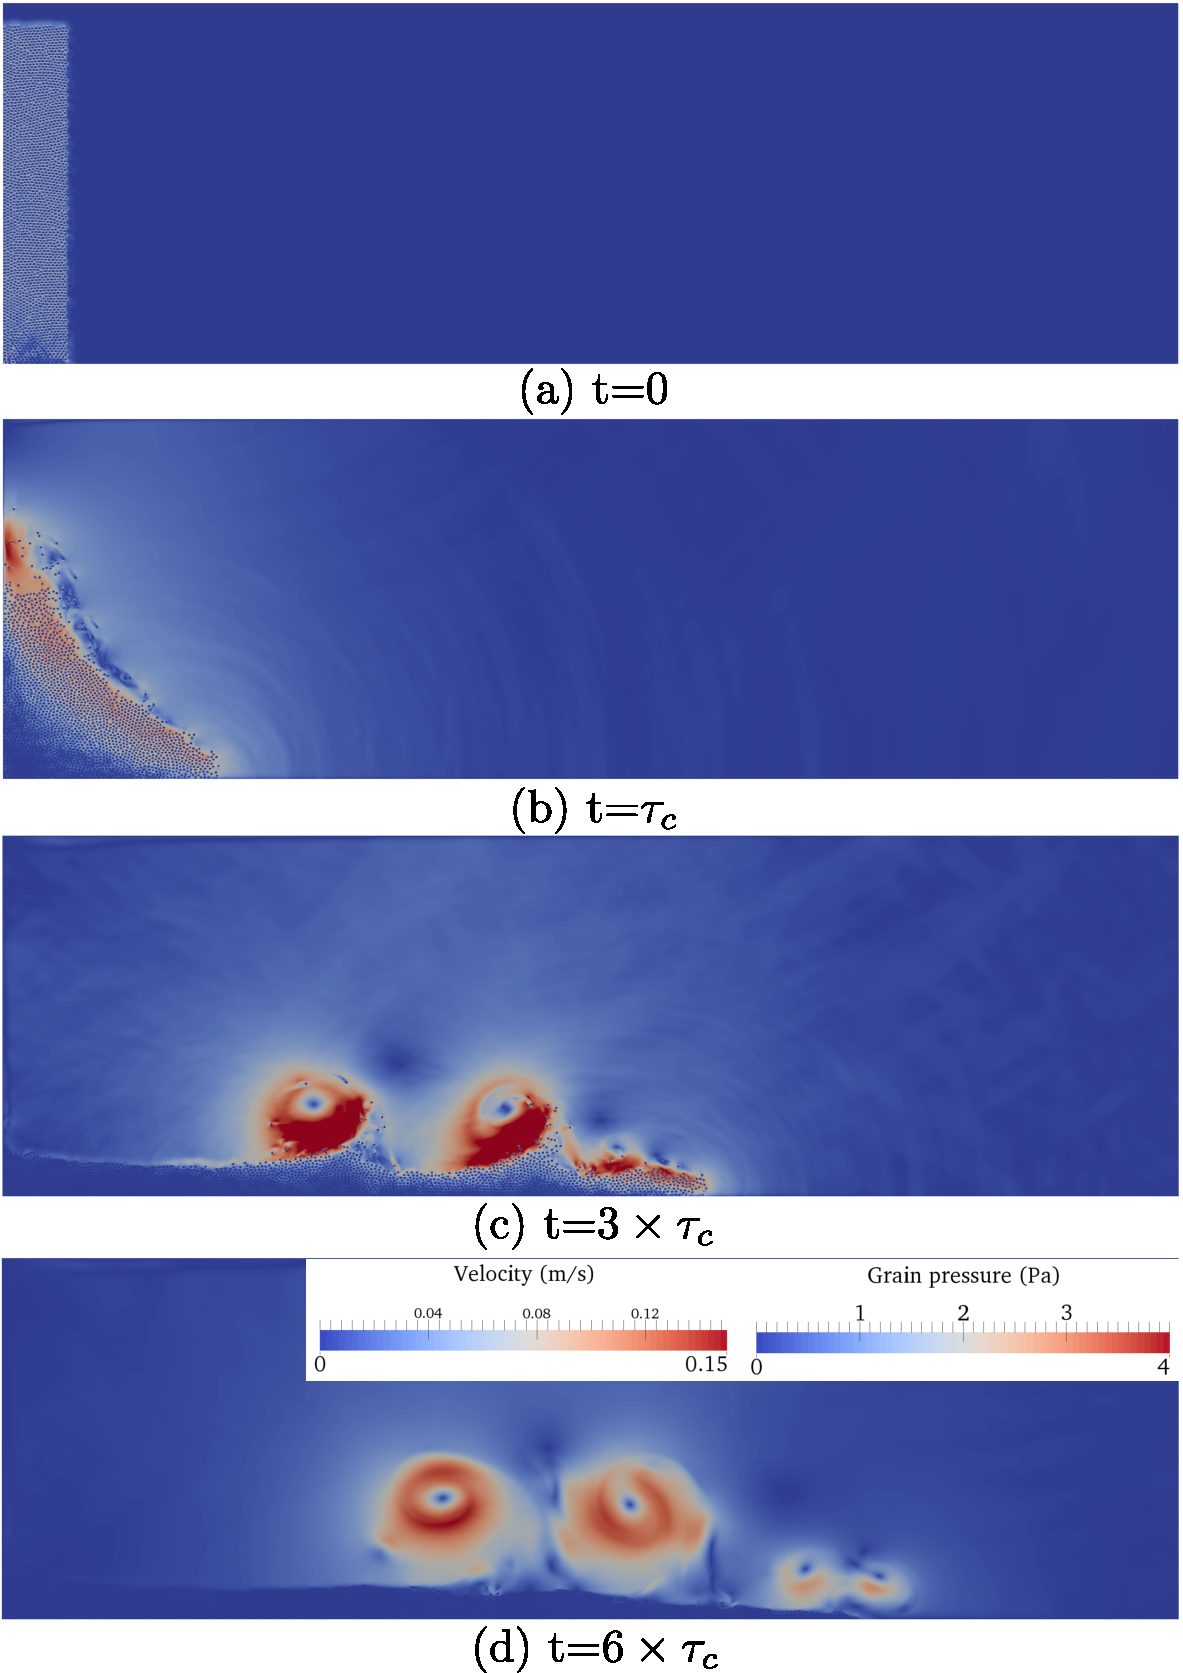
\includegraphics[width=0.9\linewidth]{figs/lbm_dem_a6}
\caption{Flow evolution of a granular column collapse in fluid (a = 6) on a 
horizontal surface.}
\label{fig:LBM_DEM_a6}
\end{figure}


Snapshots of the collapse of a granular column (\textit{a} = 6) on a inclined 
plane at angle of 5\si{\degree} are shown in~\cref{fig:a6_slope_snapshots}. 
The collapse on a slope of 5\si{\degree} show flow evolution behaviour similar 
to the case of collapse on a horizontal plane. The vortices are formed only 
during the horizontal spreading stage $t = 3\tau_c$, but the number of vortices 
formed during the collapse is higher than the collapse on a horizontal plane. 
However, as the flow progresses a single large vortex engulfs other smaller 
vortices, thus having a significant influence on the mass 
distribution.~\Cref{fig:a6_slope_voro} shows 
the distribution of mass and the packing density at $t = 6\tau_c$ and $t = 
8\tau_c$. A heap can be observed in front of the large vortex almost at the 
middle of the flow. The height of the heap formed in the middle of the granular 
flow is higher than the collapse height next to the wall. However, when the 
flow comes to rest and the vortex moves 
away from the flowing surface, the mass present in the heap gets redistributed 
(as seen at $t = 8\tau_c$). This behaviour is significantly different from that 
observed in the case of short columns. 

\begin{figure}
\makebox[\linewidth][c]{
\begin{subfigure}[b]{0.95\linewidth}
	\centering
    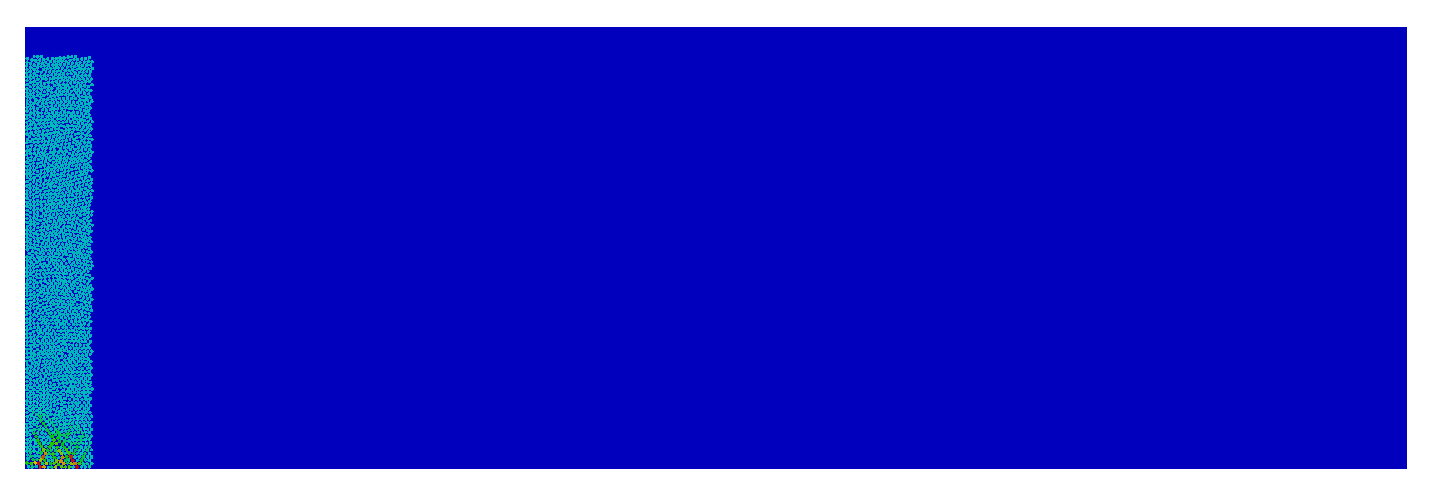
\includegraphics[width=0.95\linewidth]{figs/a6/a6slope5t_0}
    \caption*{$t = 0\tau_c$}
    \label{fig:a6slope5t_0}
\end{subfigure}
}\\

\makebox[\linewidth][c]{
\begin{subfigure}[b]{0.95\linewidth}
	\centering
    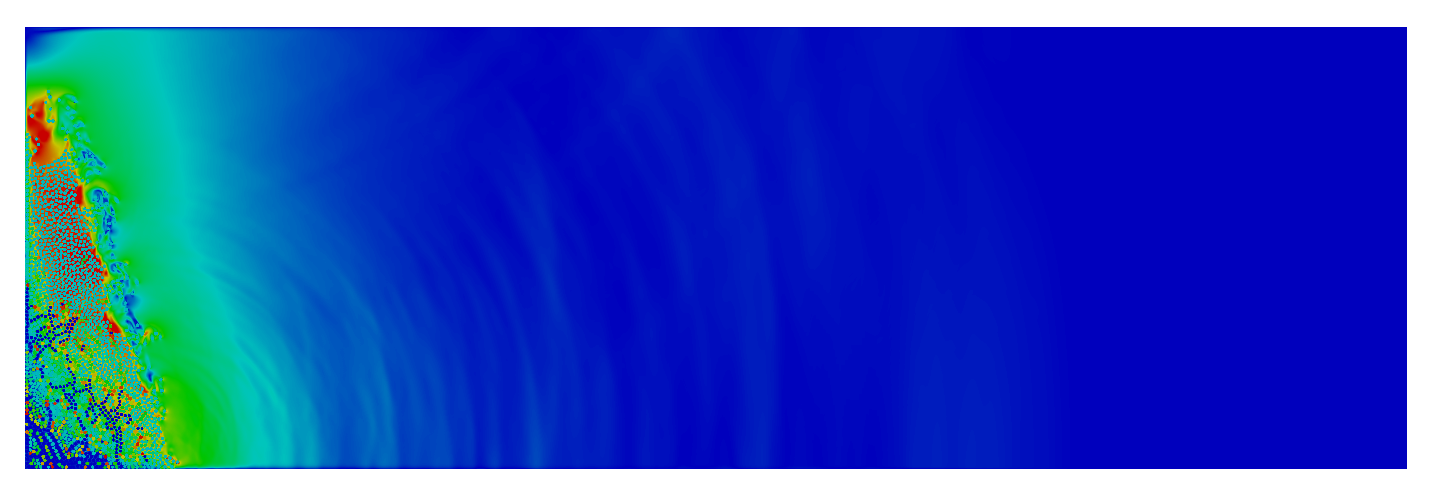
\includegraphics[width=0.95\linewidth]{figs/a6/a6slope5t_1tc}
    \caption*{$t = 1\tau_c$}
    \label{fig:a6slope5t_1tc}
\end{subfigure}
}\\

\makebox[\linewidth][c]{
\begin{subfigure}[b]{0.95\linewidth}
	\centering
    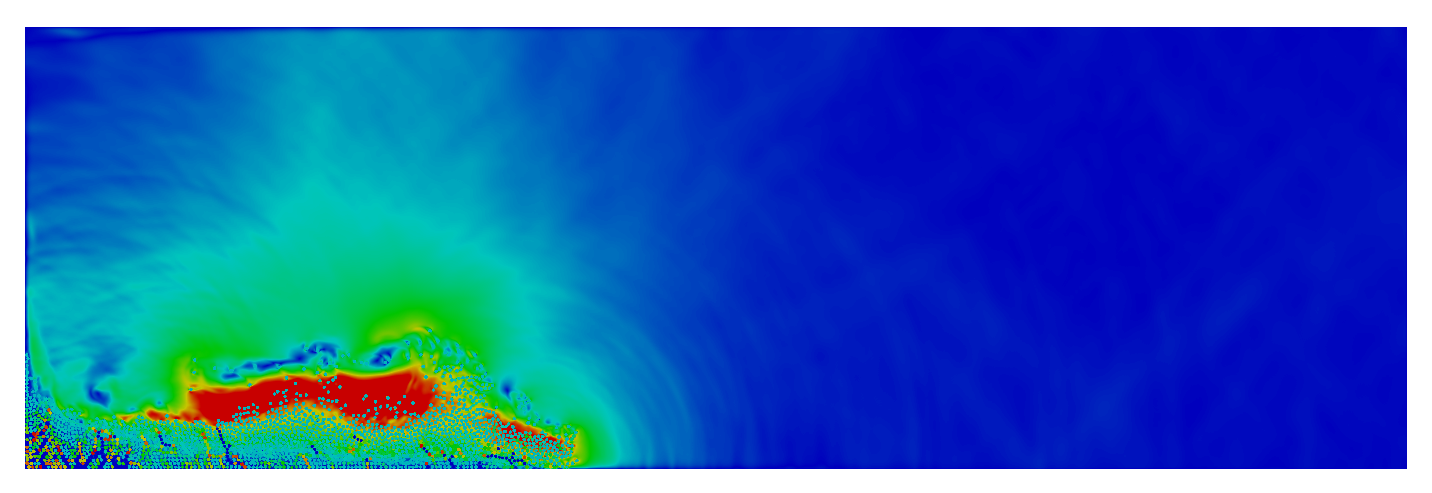
\includegraphics[width=0.95\linewidth]{figs/a6/a6slope5t_3tc}
    \caption*{$t = 3\tau_c$}
    \label{fig:a6slope5t_3tc}
\end{subfigure}
}\\

\makebox[\linewidth][c]{
\begin{subfigure}[b]{0.95\linewidth}
	\centering
    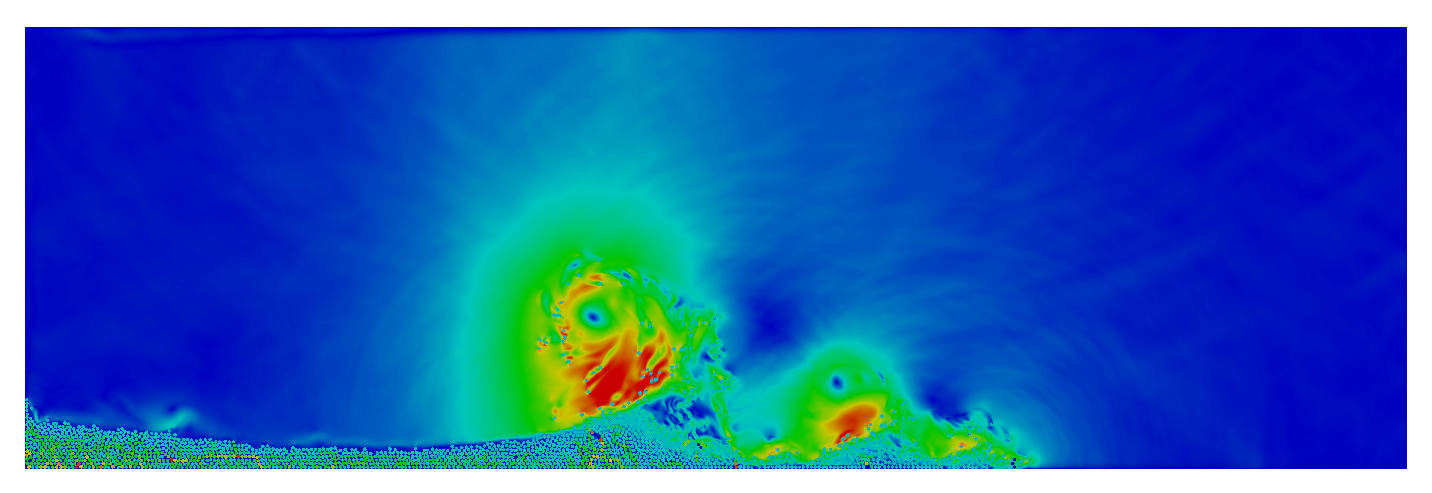
\includegraphics[width=0.95\linewidth]{figs/a6/a6slope5t_6tc}
    \caption*{$t = 6\tau_c$}
    \label{fig:a6slope5t_6tc}
\end{subfigure}
}\\

\makebox[\linewidth][c]{
\begin{subfigure}[b]{0.95\linewidth}
	\centering
    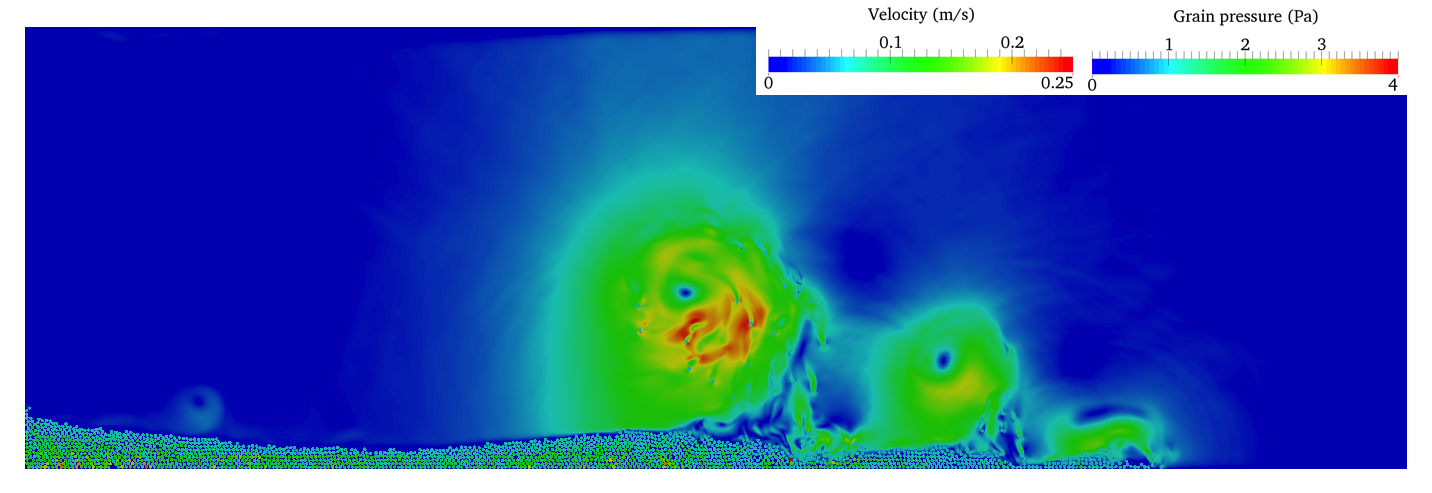
\includegraphics[width=0.95\linewidth]{figs/a6/a6slope5t_8tc}
    \caption*{$t = 8\tau_c$}
    \label{fig:a6slope5t_8tc}
\end{subfigure}
}
\caption[Flow evolution of a granular column collapse in fluid (a = 6) on a 
slope of 5\si{\degree}]{Flow evolution of a granular column collapse in fluid 
(a = 6) on a slope of 5\si{\degree}. Shows the velocity profile of fluid due to 
interaction with the grains (red - higher velocity).}
\label{fig:a6_slope_snapshots}
\end{figure}



\begin{figure}
\makebox[\linewidth][c]{
\begin{subfigure}[b]{0.95\linewidth}
	\centering
    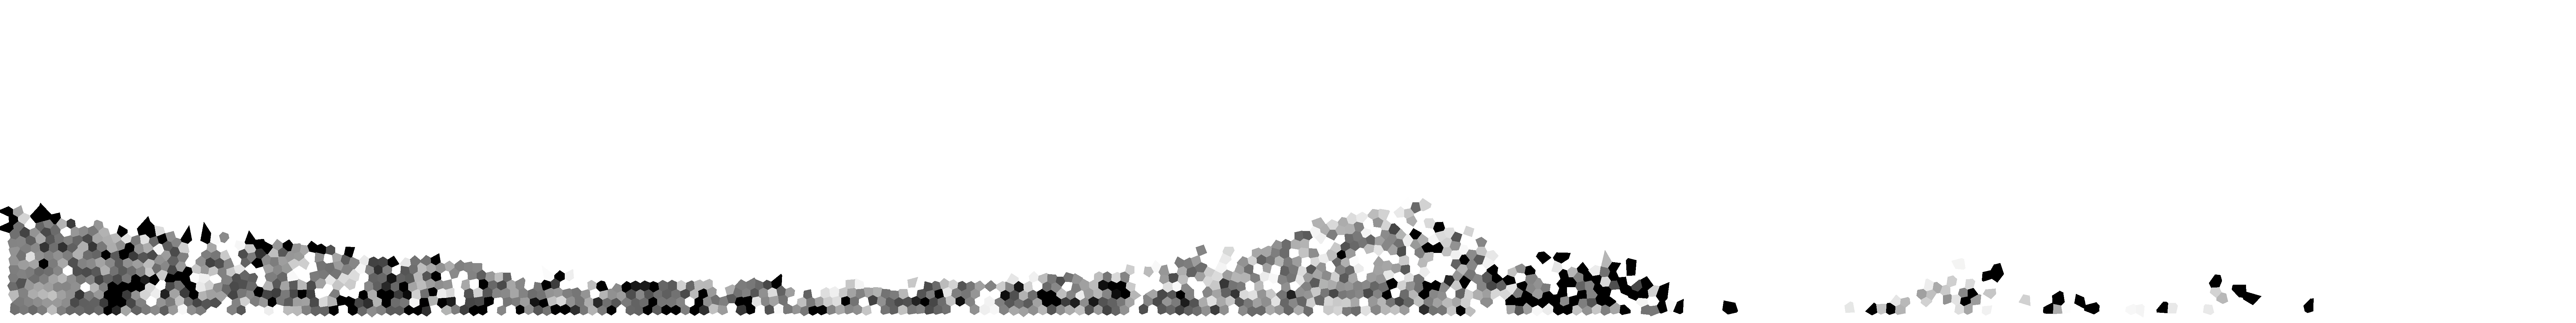
\includegraphics[width=0.95\linewidth]{figs/a6/a6_slope5_6tc}
    \caption*{$t = 6\tau_c$}
    \label{fig:a6_slope5_6tc}
\end{subfigure}
}\\
\makebox[\linewidth][c]{
\begin{subfigure}[b]{0.95\linewidth}
	\centering
    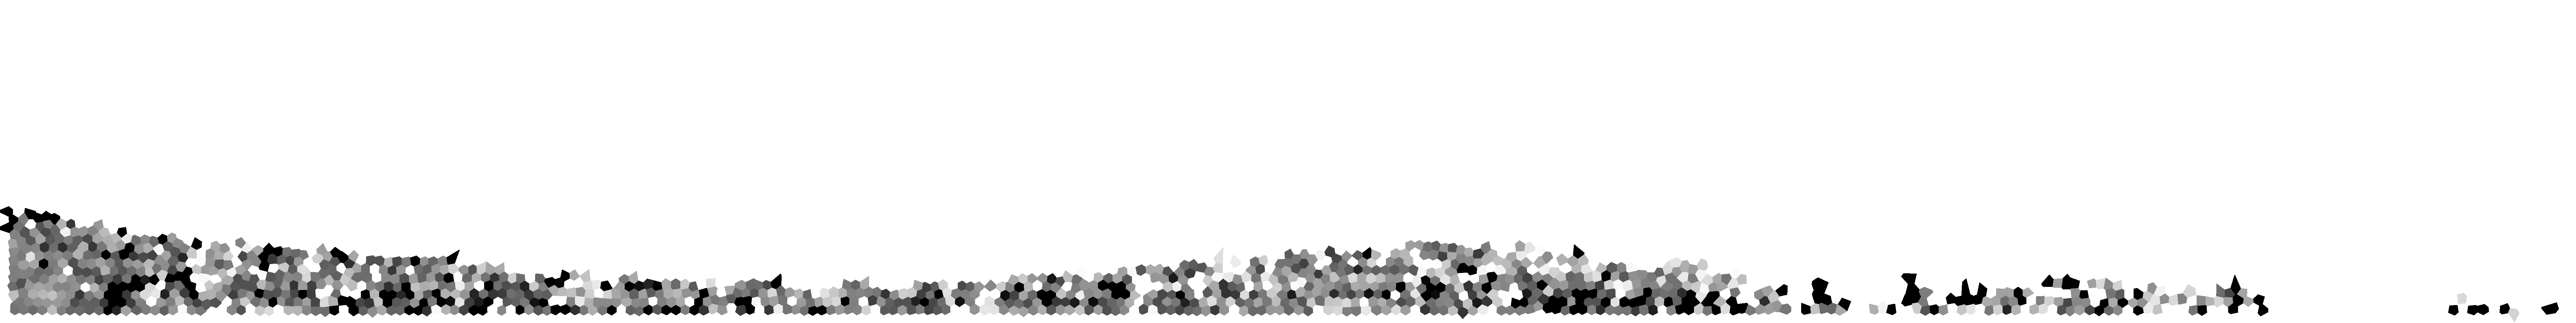
\includegraphics[width=0.95\linewidth]{figs/a6/a6_slope5_8tc}
    \caption*{$t = 8\tau_c$}
    \label{fig:a6_slope5_8tc}
\end{subfigure}
}
\caption{Packing density of a granular column collapse in fluid (a = 6) on a 
slope of 5\si{\degree}.}
\label{fig:a6_slope_voro}
\end{figure}


In order to understand the influence of slope angles on the run-out behaviour, 
the collapse of a granular column with an initial aspect ratio of 6 is 
performed on slopes of 0\si{\degree}, 2.5\si{\degree}, 5\si{\degree} and 
7.5\si{\degree}. The run-out evolution with time for different slope angles are 
presented in~\cref{fig:Runout_a6_slope}. The run-out distance increases with 
increase in the slope angle, however the run-out distance in the fluid is 
significantly shorter than the dry condition. The slow evolution of run-out in 
the submerged condition is due to the delay in the dissipation of large 
negative pore-pressures developed during the initial stage of the collapse. The 
formation of eddies during the flow indicates that most of the potential energy 
gained during the free-fall is dissipated through viscous drag and turbulence. 
This effect predominates over the hydroplaning that is observed during 
the flow resulting in a shorter run-out distance in the case of fluid. The 
evolution of the normalised height with time (\cref{fig:Height_a6_slope}) for 
collapse on different slope angles indicates that the 
amount of material destabilised in fluid is less than the dry conditions due to 
the drag forces experienced by the grains, which retards the quantity and the 
rate of collapse.

\begin{figure}
\centering
\begin{subfigure}[t]{0.9\linewidth}
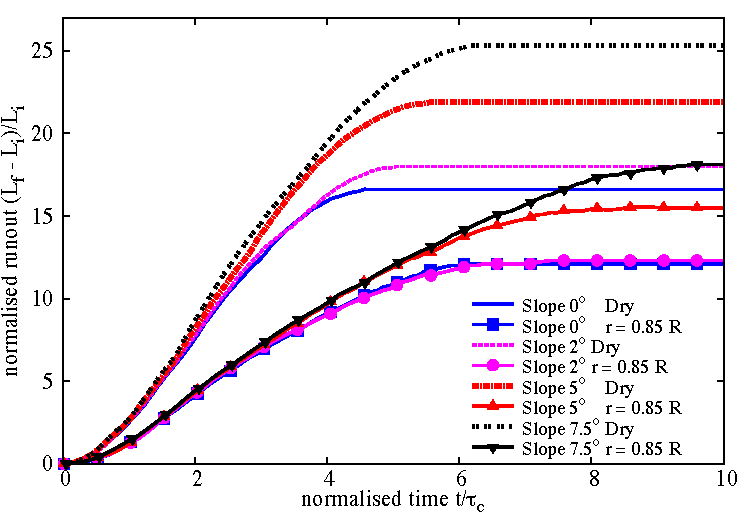
\includegraphics[width=0.9\linewidth]{figs/runout_a6_slope}
\caption{Evolution of run-out for a column collapse in fluid (a = 6).}
\label{fig:Runout_a6_slope}
\end{subfigure} \\
\begin{subfigure}[t]{0.9\linewidth}
\centering
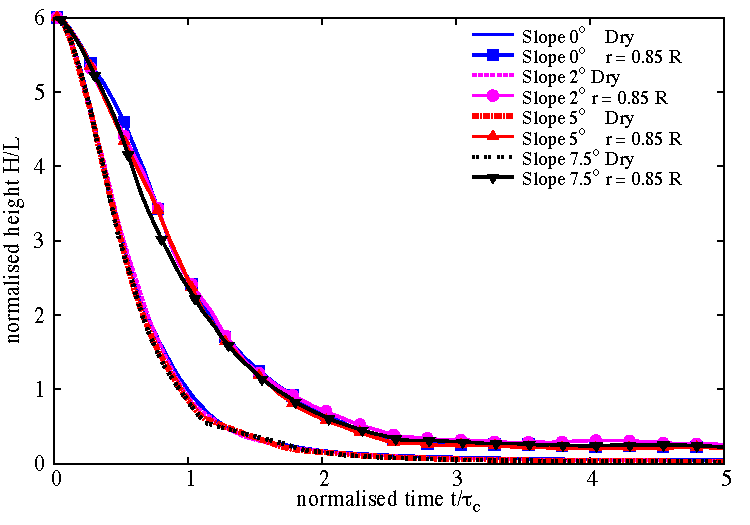
\includegraphics[width=0.9\linewidth]{figs/height_a6_slope}
\caption{Evolution of height with time for a column collapse in fluid (a = 6).}
\label{fig:Height_a6_slope}
\end{subfigure}
\caption{Evolution of  run-out and height  for a column collapse in fluid (a = 
6).}
\label{fig:a6_slope}
\end{figure}

\Cref{fig:KE_a6_slope} shows the evolution of the normalised kinetic energy 
for a granular column (a = 6) collapse in fluid on different slope angles. The 
amount of kinetic energy available for the flow in the submerged condition 
is almost half that of the dry condition. It can be seen from the figure that 
the vertical kinetic energy in the fluid condition dissipates a longer 
duration, in contrast to the free-fall release observed in the dry condition. 
The slower dissipation is attributed to the viscous drag force experienced by 
the grains. 

\begin{figure}
\centering
\makebox[\linewidth][c]{
\begin{subfigure}[t]{0.8\linewidth}
	\centering
    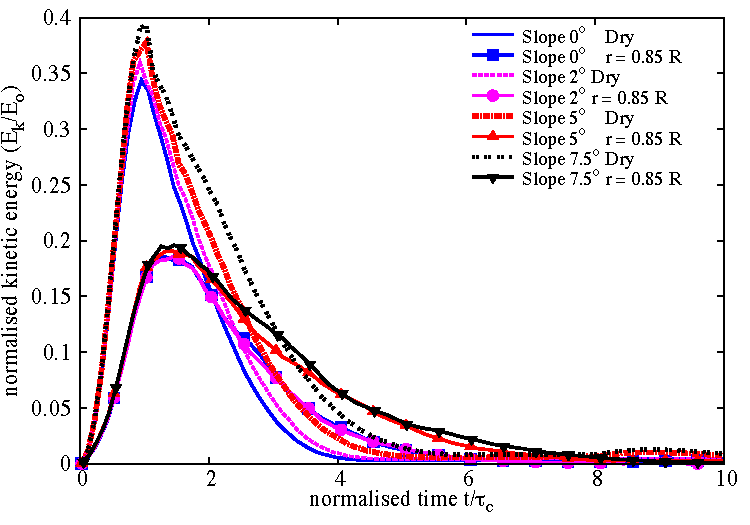
\includegraphics[width=\linewidth]{figs/KE_a6_slope}
    \caption{Evolution of the total kinetic energy.}
    \label{fig:KE_a6_slope}
\end{subfigure}
}\\
\makebox[\linewidth][c]{
\begin{subfigure}[t]{0.95\linewidth}
	\centering
    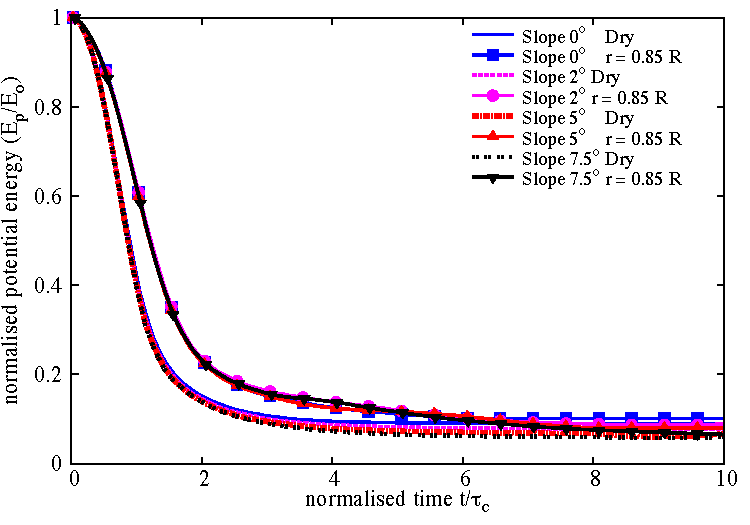
\includegraphics[width=\linewidth]{figs/PE_a6_slope}
    \caption{Evolution of the total potential energy.}
    \label{fig:PE_a6_slope}
\end{subfigure}
}
\caption{Evolution of the kinetic and the potential energy with time for a 
granular column collapse in fluid (a = 6).}
\label{fig:a6_KEPE}
\end{figure}


\begin{figure}
\centering
\makebox[\linewidth][c]{
\begin{subfigure}[t]{0.8\linewidth}
	\centering
    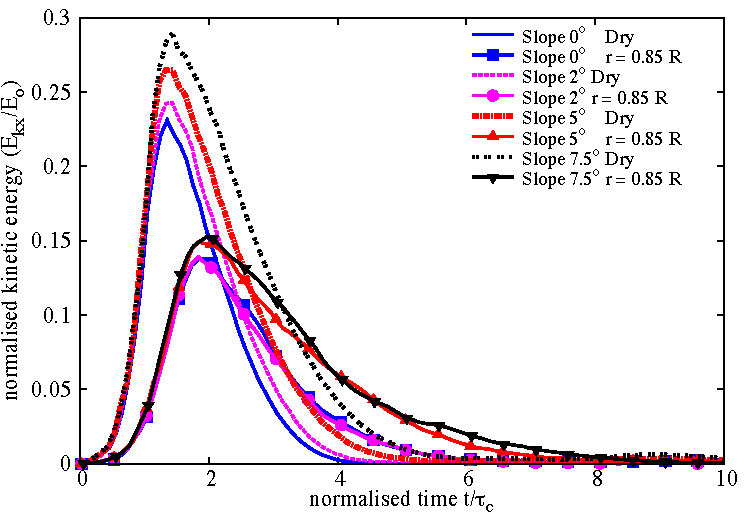
\includegraphics[width=\linewidth]{figs/KEx_a6_slope}
    \caption{Evolution of the horizontal kinetic energy.}
    \label{fig:KEx_a6_slope}
\end{subfigure}
}\\
\makebox[\linewidth][c]{
\begin{subfigure}[t]{0.95\linewidth}
	\centering
    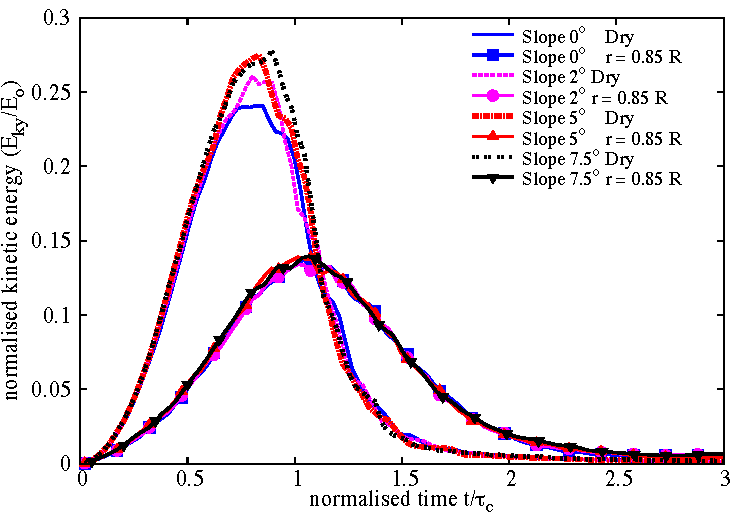
\includegraphics[width=\linewidth]{figs/KEy_a6_slope}
    \caption{Evolution of the vertical kinetic energy.}
    \label{fig:KEy_a6_slope}
\end{subfigure}
}
\caption{Evolution of the kinetic energies with time for a granular 
column collapse in fluid (a = 6).}
\label{fig:a6_KExy}
\end{figure}

The behaviour of tall columns is significantly different from that observed in 
the case of short columns. The slope angle has a strong influence on the number 
and size of eddies during the flow. The eddies interact with the surface of the 
granular flow and forms heaps in front of each vortex. This significantly 
affects the mass distribution and in turn the run-out evolution. Although tall 
cliffs are quite rare in submarine condition in comparison to short cliffs or 
slopes, further research is required to understand the influence of 
permeability and packing density on the run-out evolution of tall columns. 



\section*{Acknowledgements}
The author would like to thank the Cambridge Commonwealth and Overseas Trust for the financial support to the
first author to pursue this research.

%
% BibTeX or Biber users please use (the style is already called in the class, ensure 
% that the "woc.bst" style is in your local directory)
% \bibliography{name or your bibliography database}
%
% Non-BibTeX users please use
%
\bibliography{references} 

\end{document}

% end of file template.tex
